\chapter{Results and discussion}

\shorthandoff{-} 

\section{Cloned \tax{promoter::GFP} sequences}
As most of the strains listed in the Table \ref{strains} were prepared several years ago and not by myself, we wanted to check which parts of the promoters we actually have cloned upstream of GFP gene in those cells.
For this purpose I designed pUA66\textunderscore insert primers (Table \ref{pcr}) based on the pUA66 and pU139 vector sequences (\hyperlink{pUA66seq}{Appendix 1} and \hyperlink{pUA66seq}{Appendix 2}).
PCR products were sequenced by Macrogen, Korea using Sanger platform.

\hypertarget{SeqRes}{\subsection{\tax{placZ::GFP} strains}}
In the Fig. \ref{placZ} we can see that SC1\textunderscore D9 and MG1655 differ in \tax{lacZ} promoter region by a single SNP at position 39 nt upstream from \tax{lacZ} gene start codon (position 199 in Fig. \ref{placZ}).
These 2 strains have 3 more SNPs further downstream in \tax{lacZ} gene itself 
(positions 306, 324 and 363 in Fig. \ref{placZ}).
Based on the alignment of acquired \tax{lacZ} promoters sequences (Fig. \ref{placZ}) we can confirm that those assumed to originate from SC1\textunderscore D9 have an appropriate sequence as well as for MG1655.
\begin{figure}[ht]
  \centering
  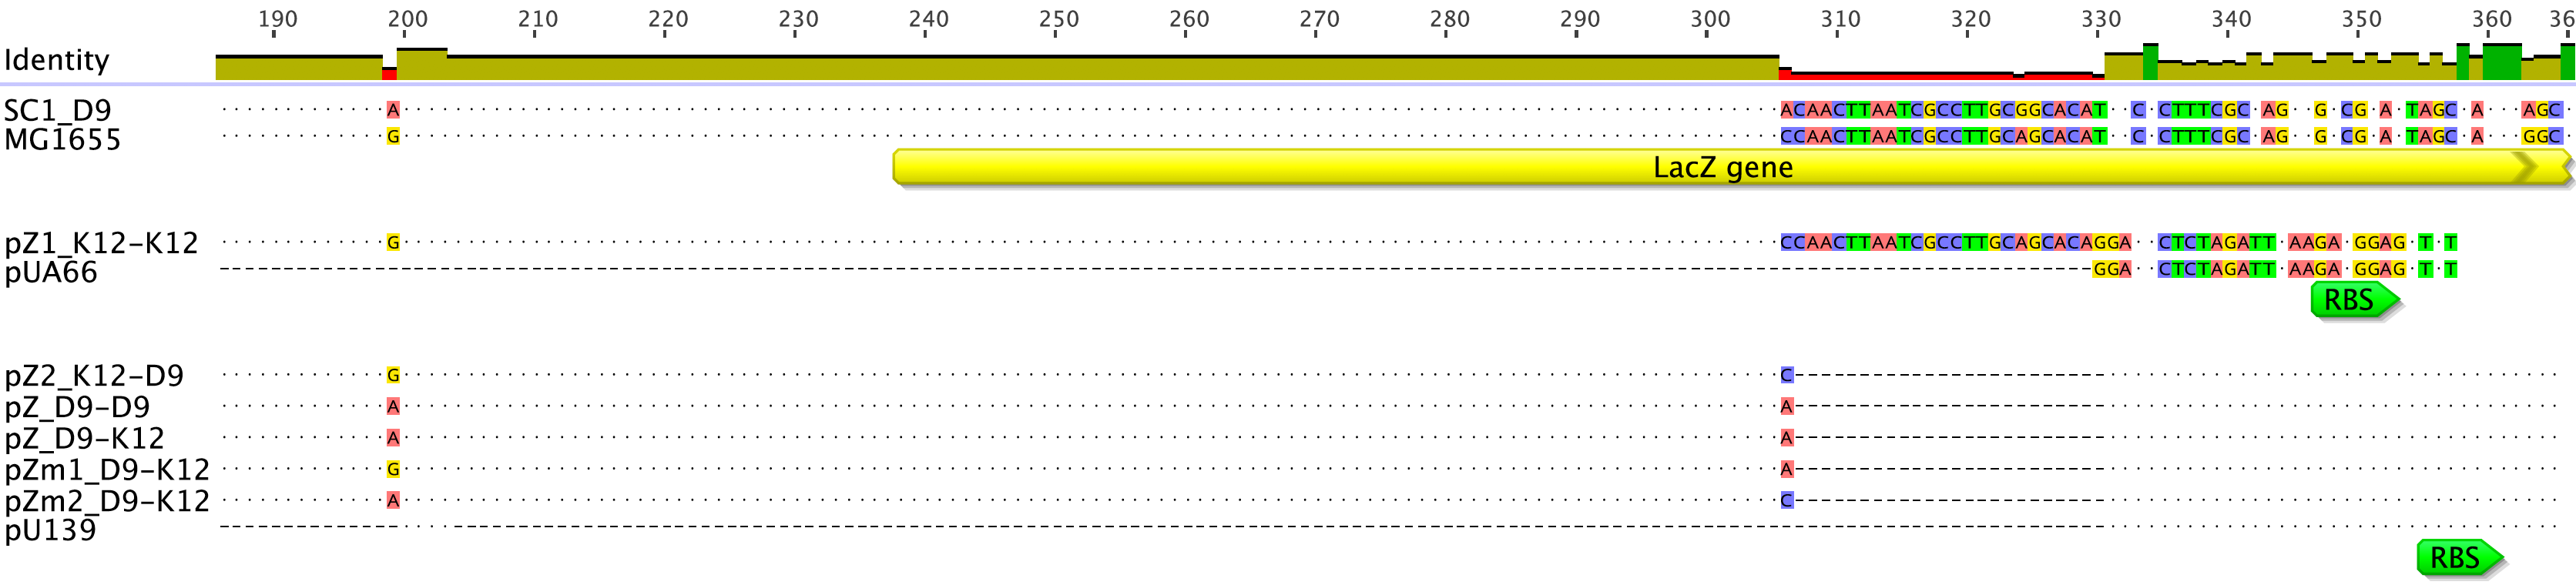
\includegraphics[scale=0.25]{text/Pictures/placZsequences.png}
	\caption{Excerpt of \tax{lacZ} promoters alignment with vectors and references. SC1\textunderscore D9 and MG1655 are reference sequences of \tax{lacZ} promoters from particular strains. pUA66 and pU139 are vectors aligned with no promoter upstream of GFP gene (not shown).}
	\label{placZ}
\end{figure}
Beside the SNPs in \tax{lacZ} promoter, the first SNP from \tax{lacZ} coding sequence is included in all vectors upstream of GFP.
Most of the strains possess pU139 as the vector except for pZ1\textunderscore K12-K12 which was acquired from Alon library \cite{zaslaver2006comprehensive}.
This strain have also longer part of \tax{lacZ} gene cloned into its pUA66 vector, potentially covering second SNP in it when compared to SC1\textunderscore D9.
This is not the only difference of pZ1\textunderscore K12-K12, as part of the \tax{lacI} gene is incorporated in all sequences listed in Fig. \ref{placZ} on the opposite site of the promoter (\hyperlink{placZalign}{Appendix 3}) and pZ1\textunderscore K12-K12 has this \tax{lacI} sequence almost 60 bp shorter than the rest of these strains.
Note, that strain pZ1m1\textunderscore D9-K12 and pZ1m2\textunderscore D9-K12 possess a recurrent mutation of the SNP in \tax{lacZ} promoter or \tax{lacZ} gene, respectively (from SC1\textunderscore D9 back to MG1655).
You can also realize that strain pZ2\textunderscore K12-K12 is not included in the Fig. \ref{placZ}.
The reason is that it was made by transforming the plasmid from pZ2\textunderscore K12-D9 into MG1655 after receiving the sequencing data and was not sequenced afterwards.

\subsection{\tax{precA::GFP} strains}
Both pA\textunderscore K12-K12 and pA\textunderscore K12-D9 strains have the same plasmid (pU139) as the latter was made by transforming plasmid from the former.
It was also confirmed by sequencing as well as that the sequence upstream of GFP gene correspond to \tax{recA} promoter of MG1655 (\hyperlink{precAalign}{Appendix 4}).
Similar to the cloned \tax{lacI}-\tax{lacZ} intergenic regions mentioned above, the sequence incorporated into pU139 and then transformed into these \tax{precA::GFP} strains includes parts of \tax{recA} gene downstream and \tax{pncC} gene upstream of the very promoter.


\section{Ciprofloxacin susceptibility}
Because we want to induce \tax{recA} promoter by exposing the cells to a sub-lethal (i.e. sub-MIC) exposure to Ciprofloxacin, I had to make sure the strains I use are susceptible to Ciprofloxacin, first.
I wanted also to estimate what are the minimum inhibitory concentrations (MICs) for this antibiotic in the strains used.
MG1655 and SC1\textunderscore D9 were incubated in an increasing concentration of Ciprofloxacin (see \hyperlink{MIC}{Materials and Methods}).
\begin{figure}[b!]
  \centering
  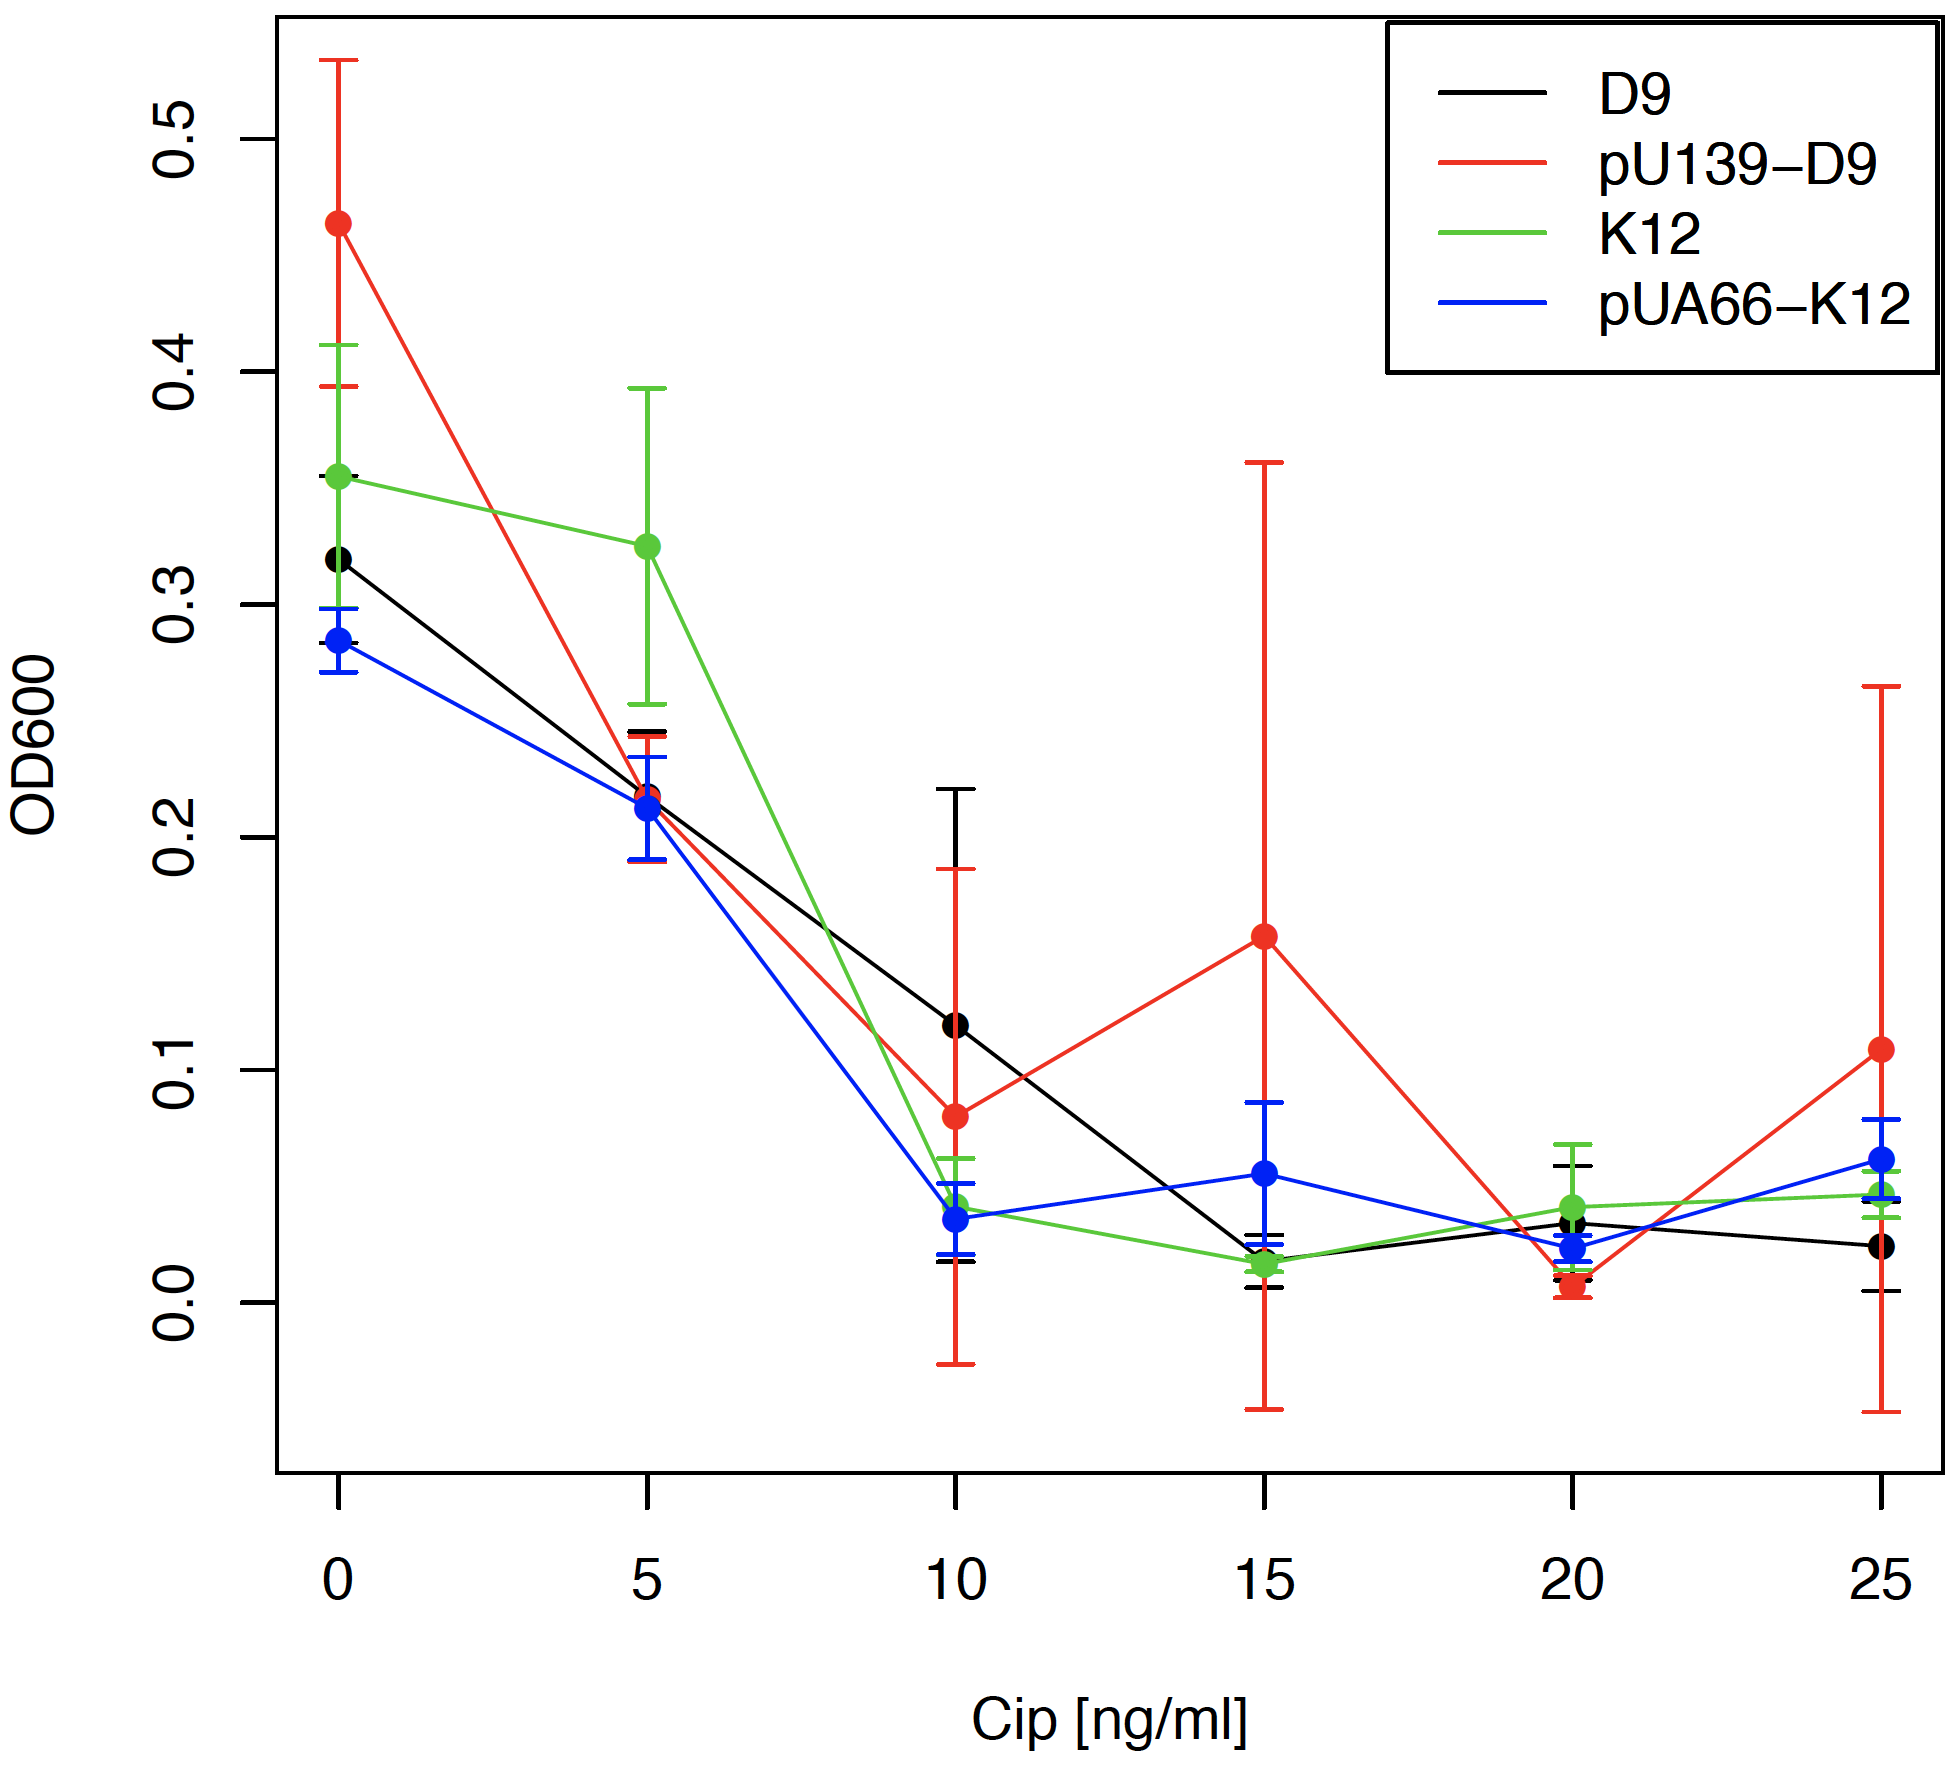
\includegraphics[scale=0.25]{text/Pictures/KillCurve.png}
	\caption{Cell density after 24 h growth of MG1655 and SC1\textunderscore D9 strains in various Ciprofloxacin concentrations. Strains with a promoter-less plasmid are also included.}
	\label{killing}
\end{figure}
Strains with promoter-less pU139 or pUA66 plasmid were also included to ensure the Kanamycin resistance carried on the plasmid does not affect Ciprofloxacin sensitivity.
The MIC for both strains is 10 ng/ml of Ciprofloxacin or less, however 5 ng/ml is the concentration which both strains are able to survive, although a decrease in the final cell density is observed when compared to the growth in the absence of Ciprofloxacin (Fig. \ref{killing}).
Plasmid carried Kanamycin resistance causes none or small effect on Ciprofloxacin susceptibility.


\section{Variation in promoter activity}
To explore the differences in promoter activity and genetic backgrounds, 4 h cultures grown in M9 minimal media with a single carbon source were assayed using flow cytometry (see \hyperlink{FC}{Materials and Methods}).
Exported FCS files were then analysed in R - used scripts are available at \href{https://github.com/marketavlkova/}{GitHub} repositories.

\subsection{Activity of \tax{lacZ} promoters}
\phantomsection%%% removes warning: "package hyperref warning the anchor of a bookmark and its parent's must not be the same. Added a new anchor on input line 55."
\subsubsection{Expression in lactose environment}
All strains with \tax{lacZ} promoter cloned upstream of GFP gene and strain ASC662, which has GFP integrated into chromosome in \tax{lac} operon, show strong GFP expression when grown in lactose as a sole carbon source (Fig. \ref{lacZassay}).
All plasmid based models show about 2.5 to 10.5 times (3.842 au $\pm$ 0.113 in pZ1\textunderscore K12-K12 to 4.464 au $\pm$ 0.095 in pZm1\textunderscore D9-K12) higher GFP expression than ASC662 (3.442 au $\pm$ 0.140).
Expression differences are also observed when a promoter sequences of the same length, but originating from different strains (2 SNPs present) are cloned into the same genotypic background.
Strain pZ\textunderscore D9-D9 has over 1.5 times higher mean GFP expression than pZ2\textunderscore K12-D9 (4.403 au $\pm$ 0.202 and 4.219 au $\pm$ 0.134, respectively).
Similarly, pZ\textunderscore D9-K12 has almost 1.5 times higher mean expression than pZ2\textunderscore K12-K12 (4.437 au $\pm$ 0.117 and 4.267 au $\pm$ 0.103, respectively).
Over 2.5-fold difference in expression is also observed when comparing both strains with two versions of cloned promoter sequence both originating from MG1655 into the same strain, i.e. pZ1\textunderscore K12-K12 and pZ2\textunderscore K12-K12.
The former having mean expression 3.842 au $\pm$ 0.113, the latter 4.267 au $\pm$ 0.103.
We think this is caused by differences in 5' end of the produced mRNA between these two plasmid models, which might have effect on the mRNA stability or translation efficiency.

\begin{figure}[ht!]
  \centering
  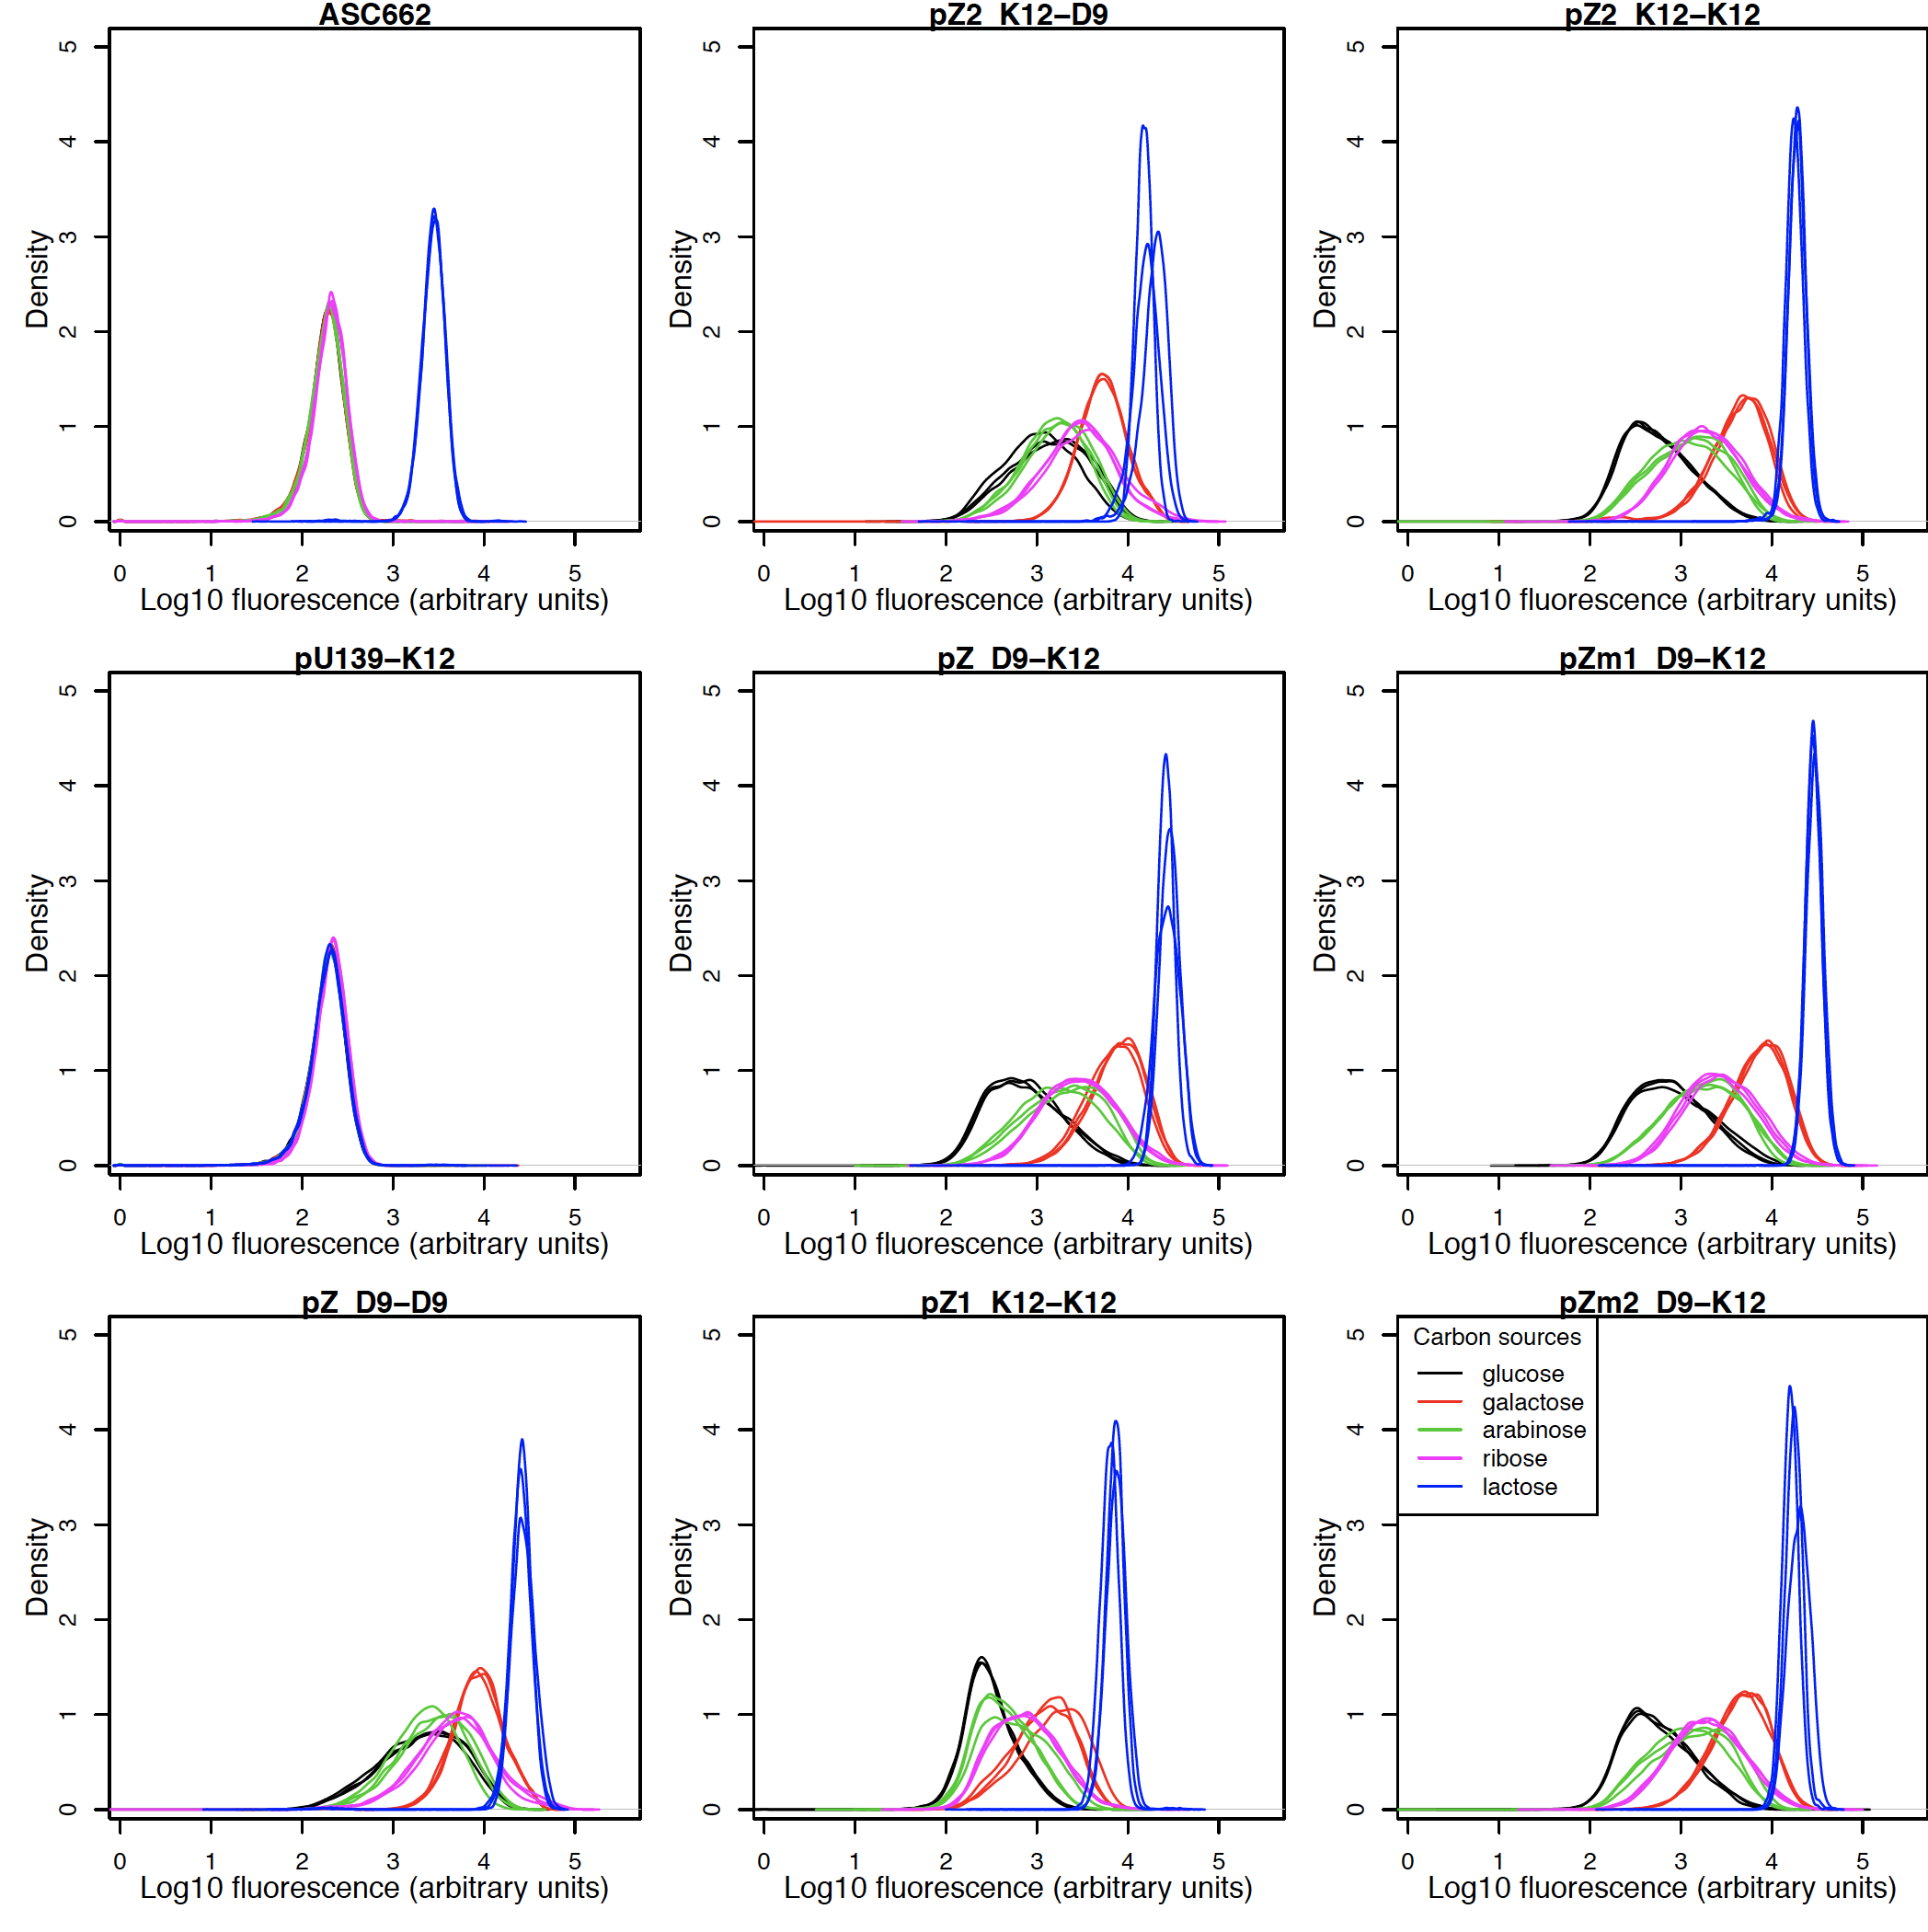
\includegraphics[scale=0.4]{text/Pictures/lacZassay.png}
	\caption{\tax{lacZ} promoter activity in various carbon sources. Strain ASC662 has GFP gene integrated into chromosome in \tax{lac} operon native locus. pU139-K12 is negative control of GFP expression for plasmid based models - promoter-less pU139 plasmid present. The rest are strains with various \tax{lacZ} promoters cloned upstream of GFP gene in a plasmid - see Table \ref{strains}.}
	\label{lacZassay}
\end{figure}

The strains pZ\textunderscore D9-K12 and pZ2\textunderscore K12-K12 differ just by the two SNPs in the sequence cloned upstream of GFP gene, while one of the SNPs is located in the cloned part of \tax{lacZ} gene, not in the promoter itself (see \hyperlink{SeqRes}{sequencing results}).
If the SNPs from \tax{lacZ} gene had no effect on the GFP expression we should see the same expression pattern in pZm1\textunderscore D9-K12 as in pZ2\textunderscore K12-K12 (i.e. 4.267 au $\pm$ 0.103).
However, this is not the case - the recurrent mutation of the first SNP (A to G) leads to even higher mean expression difference (4.464 au $\pm$ 0.095; i.e. 1.57-fold change) than is seen when the MG1655 promoter is compared to the original sequence from SC1\textunderscore D9 (4.437 au $\pm$ 0.117; i.e. 1.48-fold change).
Interestingly we get much closer mean expression values to MG1655 promoter sequence with the recurrent mutation in the \tax{lacZ} coding sequence.
This time pZm2\textunderscore D9-K12 shows a bit lower expression level than pZ2\textunderscore K12-K12 (4.249 au $\pm$ 0.105 vs 4.267 au $\pm$ 0.103; i.e. 1.04-fold change).
Again we think this might be caused by differential mRNA stability and/or translation efficiency in the plasmid based models.
Because the second SNP, which is located in \tax{lacZ} gene itself is transcribed into 5' end of the mRNA coding GFP in our models and might thus have effect on the mRNA folding.

\subsubsection{Expression in non-lactose environments}
ASC662 does not express GFP when grown in any other carbon source used as the fluorescence levels are the same as for negative control pU139-K12.
Negative control for SC1\textunderscore D9 background i.e. pU139-D9 is comparable to pU139-K12 (\hyperlink{FCnegs}{Appendix 5}).
Interestingly some \tax{lacZ} promoter activity is observed in all plasmid model strains grown in any other carbon source, even glucose (Fig. \ref{lacZassay}).
Generally in all of them we can see the same pattern - an increasing \tax{lacZ} promoter activity based on the carbon source used: glucose $<$ arabinose $<$ ribose $<$ galactose $<$ lactose.
The difference in expression between arabinose and ribose environment is relatively small, but consistent among all strains and replicates.
Moreover the mean expression levels in all these carbon sources depends not only on the promoter variant the strain has, but also at the genetic background of the strain (see pZ\textunderscore D9-D9 vs pZ\textunderscore D9-K12 and pZ2\textunderscore K12-D9 vs pZ2\textunderscore K12-K12 in Fig. \ref{lacZassay}).
Note, that some density curves (mainly those from glucose growth) do not have the regular shape which is common for all samples from lactose growth.

Presence of the fluorescence in some of these strains even during growth on non-lactose carbon source was confirmed by time-lapse fluorescent microscopy.
You can find results from growth on glucose as a sole carbon source in \hyperlink{micro}{Appendix 6}.
The results obtained this way were assessed just visually for now.
Strain pZ1\textunderscore K12-K12 seems to have the lowest GFP expression levels as well as the smallest fraction of fluorescent cells from the analysed plasmid based models.
The other two strains pZ2\textunderscore K12-K12 and pZ2\textunderscore K12-D9 also seem to exhibit the same pattern which is seen from flow cytometry results, it is that the latter strain has higher GFP expression levels than the former one and higher fraction of fluorescent cells as well.
As negative control for GFP expression pUA66-K12 was included in the experiments as well (\hyperlink{micro}{Appendix 6}).
No fluorescence (above autofluorescence) is detectable using this approach.

We believe the disproportion in GFP expression between plasmid based models and ASC662 strain under non-lactose environments is caused by multiple copies of \tax{lacZ} promoter present in plasmid models.
Even though the plasmids used produce low copy number \cite{zaslaver2006comprehensive}, it probably exceeds the number of LacI repressors present in the cells and thus enables induction of some of the \tax{lacZ} promoters present.

\subsection{Activity of \tax{recA} promoter}
Mean GFP expression levels driven by \tax{recA} promoter are proportional to the concentration of Ciprofloxacin the cells are exposed to, as you can see in Fig. \ref{recAassay}.
\begin{figure}[ht!]
  \centering
  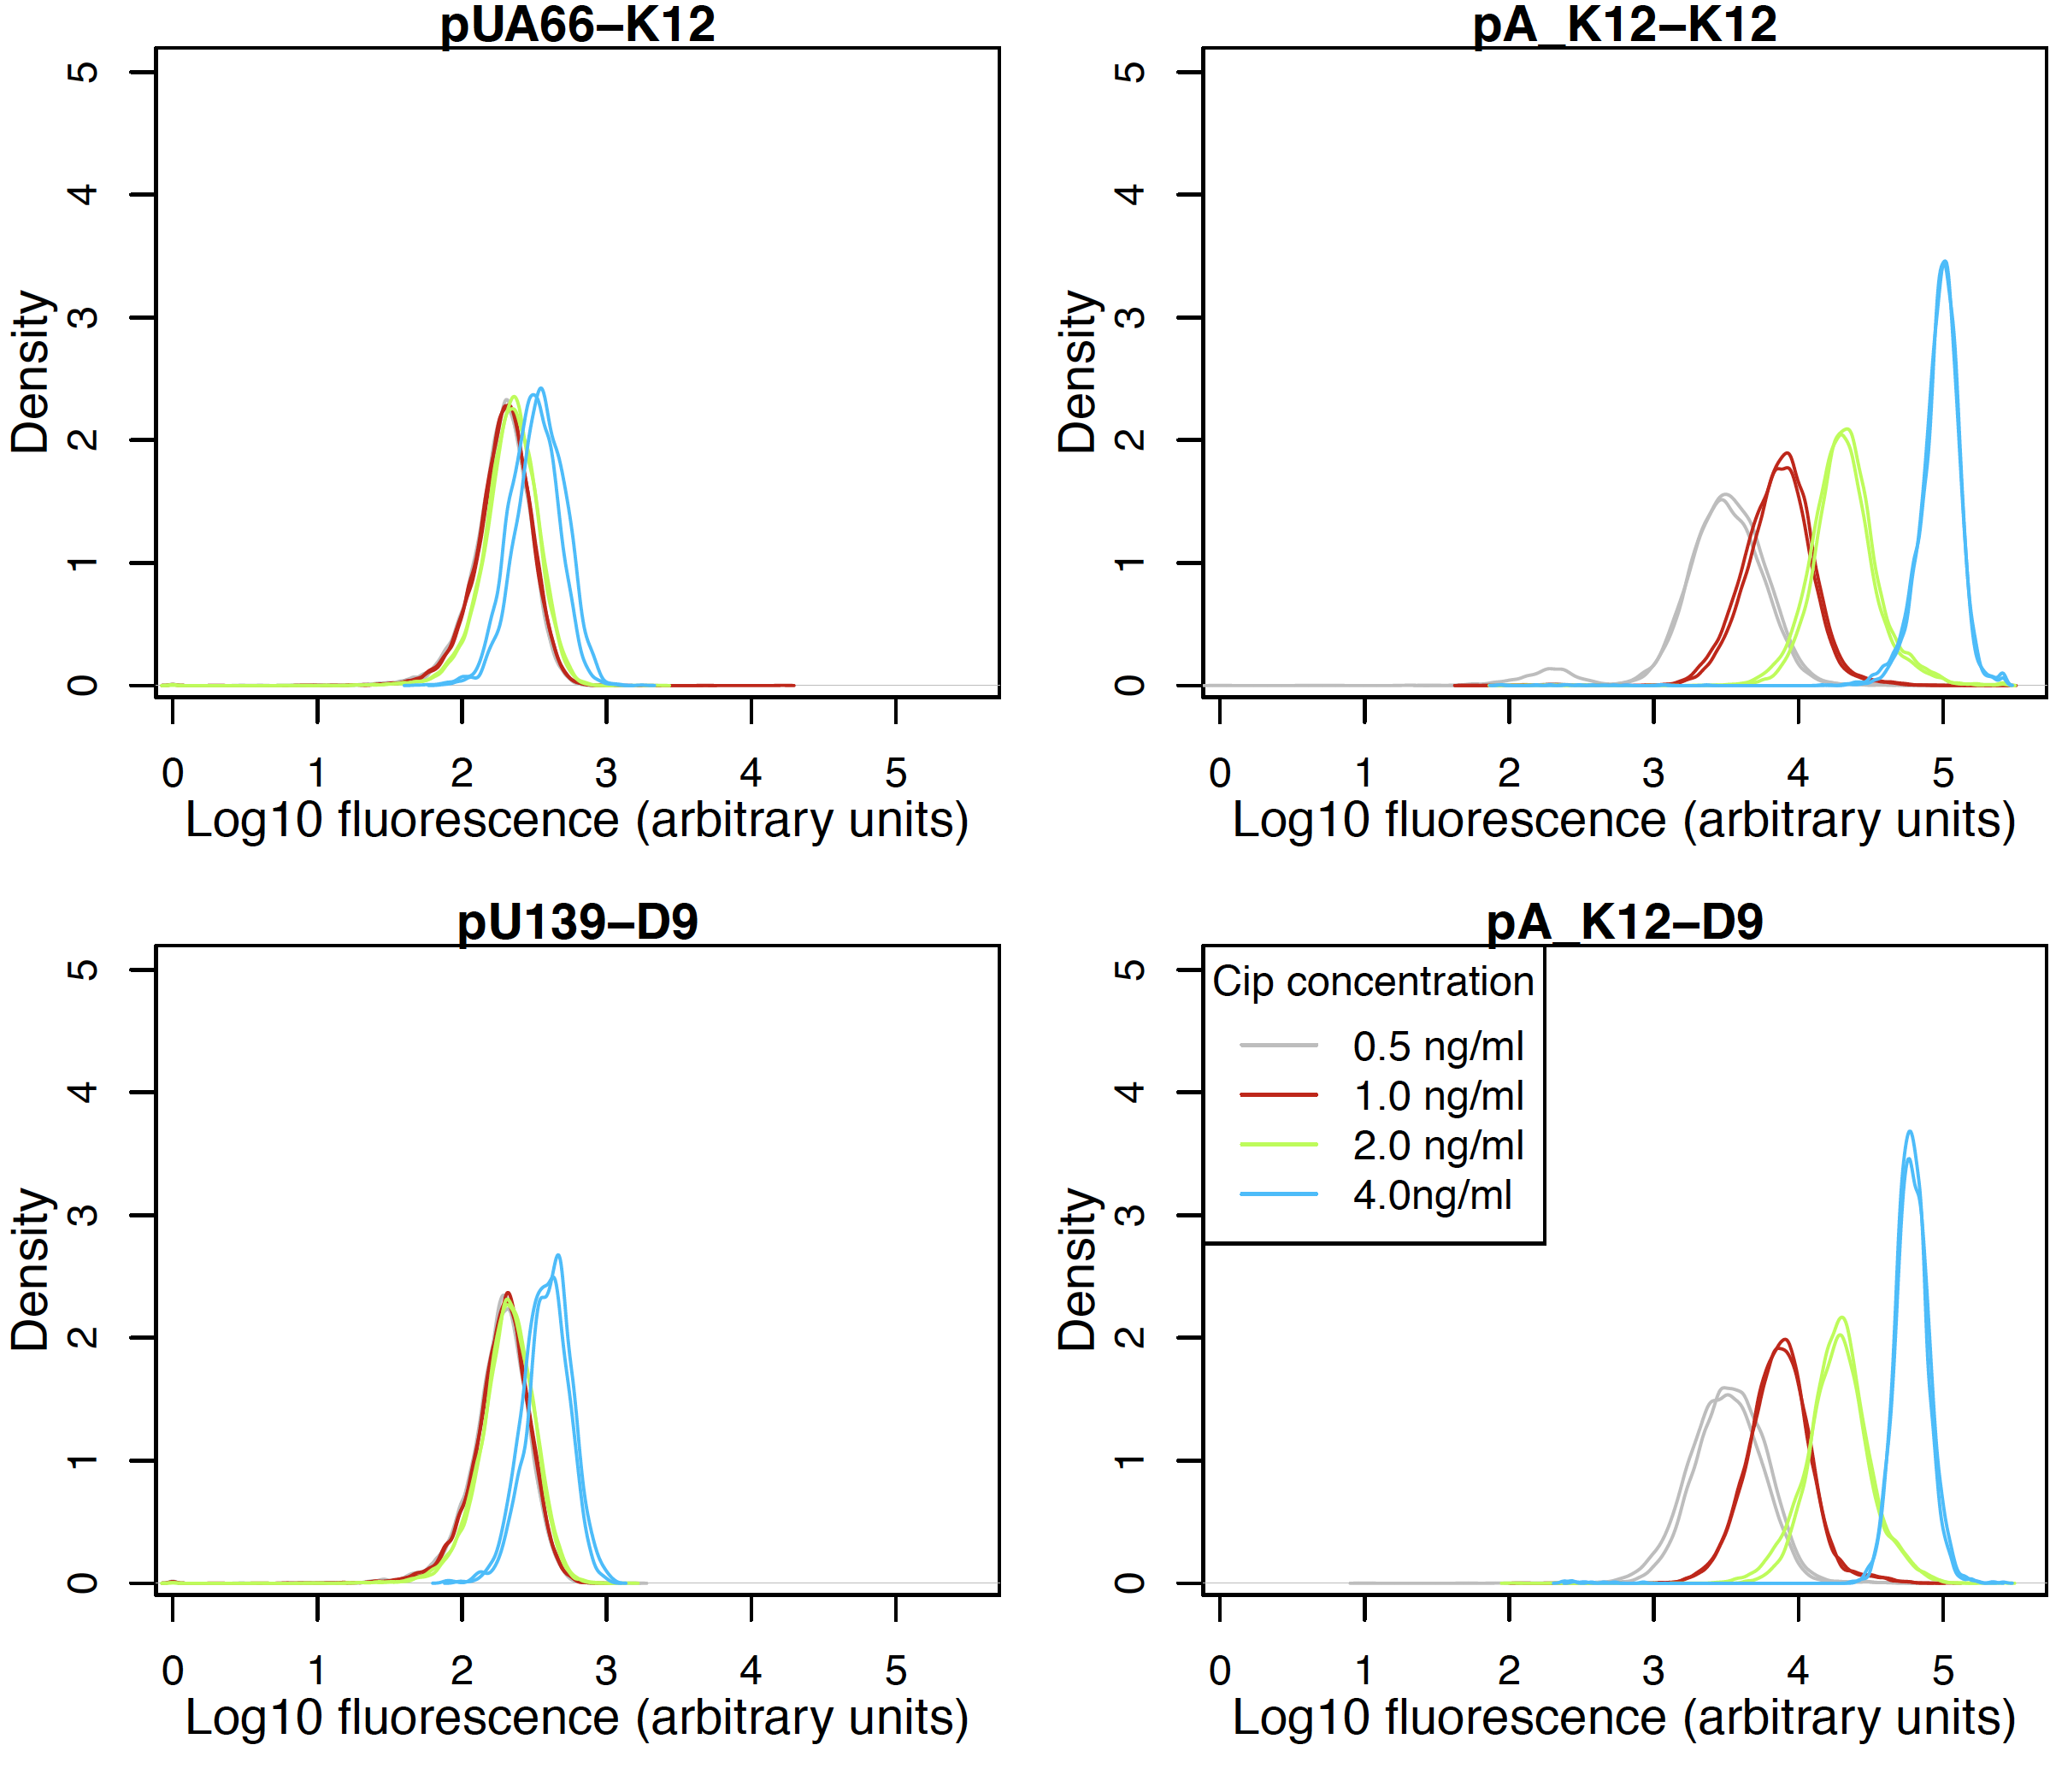
\includegraphics[scale=0.25]{text/Pictures/recAassay.png}
	\caption{\tax{recA} promoter activity in increasing concentration of Ciprofloxacin. Strains pUA66-K12 and pU139-D9 are negative controls of GFP expression for plasmid based models - promoter-less plasmid present. The rest are strains with the same \tax{recA} promoter cloned upstream of GFP gene in a plasmid - see Table \ref{strains}.}
	\label{recAassay}
\end{figure}
The induction under higher Ciprofloxacin concentrations is slightly less pronounced in pA\textunderscore K12-D9 than in pA\textunderscore K12-K12 (from 4.274 $\pm$ 0.219 to 4.779 $\pm$ 0.165, i.e. 3.20-fold change and from 4.315 $\pm$ 0.235 to 4.974 $\pm$ 0.178, i.e. 4.56-fold change from 2.0 to 4.0 ng/ml of Cip, respectively).
The mean fluorescence level is also over 1.5 times higher under 4.0 ng/ml of Ciprofloxacin in pA\textunderscore K12-K12.

Another change based on the Ciprofloxacin concentration is observed in scatter plots.
At 2.0 ng/ml of it both the forward and side scatter values of the cells begins to increase (data not shown).
This is expected to happen due to cell filamentation under higher Ciprofloxacin exposure.
It also explains the shift in fluorescence in the negative controls of GFP expression, i.e. pUA66-K12 and pU139-D9, under the highest Ciprofloxacin concentration used (Fig. \ref{recAassay}).
Interestingly, the effect of filamentation is higher in SC1\textunderscore D9 background than in MG1655 (from 2.307 $\pm$ 0.197 to 2.589 $\pm$ 0.155, i.e. 1.91-fold change and from 2.332 $\pm$ 0.193 to 2.517 $\pm$ 0.169, i.e. 1.53-fold change from 2.0 to 4.0 ng/ml of Cip, respectively), which is the opposite of what we see in \tax{recA} promoter induction.
The higher filamentation effect of SC1\textunderscore D9 is likely due to its generally smaller cells compared to MG1655.


% 17.9.2018
% where is this name from?
\section{Construction of pADOUCH plasmid}
As we could see, \tax{lacZ} promoters cloned into plasmids were active even in non-lactose environments, but that is not the case if GFP gene is integrated into chromosome.
We hypothesise, that this differential results might be caused by the naturally low amounts of LacI repressor present in a cell.
When a cell makes multiple copies of \tax{lacZ} promoter by its sequence on a plasmid, all LacI proteins become saturated and a part of the promoters escape the repression, even though the plasmids used should produce only several copies within a cell \cite{zaslaver2006comprehensive}.
To confirm that we decided to place the \tax{placZ::GFP} sequences into chromosome, creating only one additional \tax{lacZ} promoter per a cell.

We have available pLW001 plasmid which is suitable for chromosomal integration (\hyperlink{pLW001}{Appendix 7}) however, this plasmid lacks ribosome binding site (RBS).
Thus we constructed a new plasmid by replacing the GFP gene present in pLW001 vector with the GFP sequence we have in our negative control plasmid pUA66 (\hyperlink{pUA66seq}{Appendix 1}) together with its strong RBS, some additional restriction sites and a transcriptional terminator (Fig. \ref{cloning}).
\begin{figure}[ht!]
  \centering
  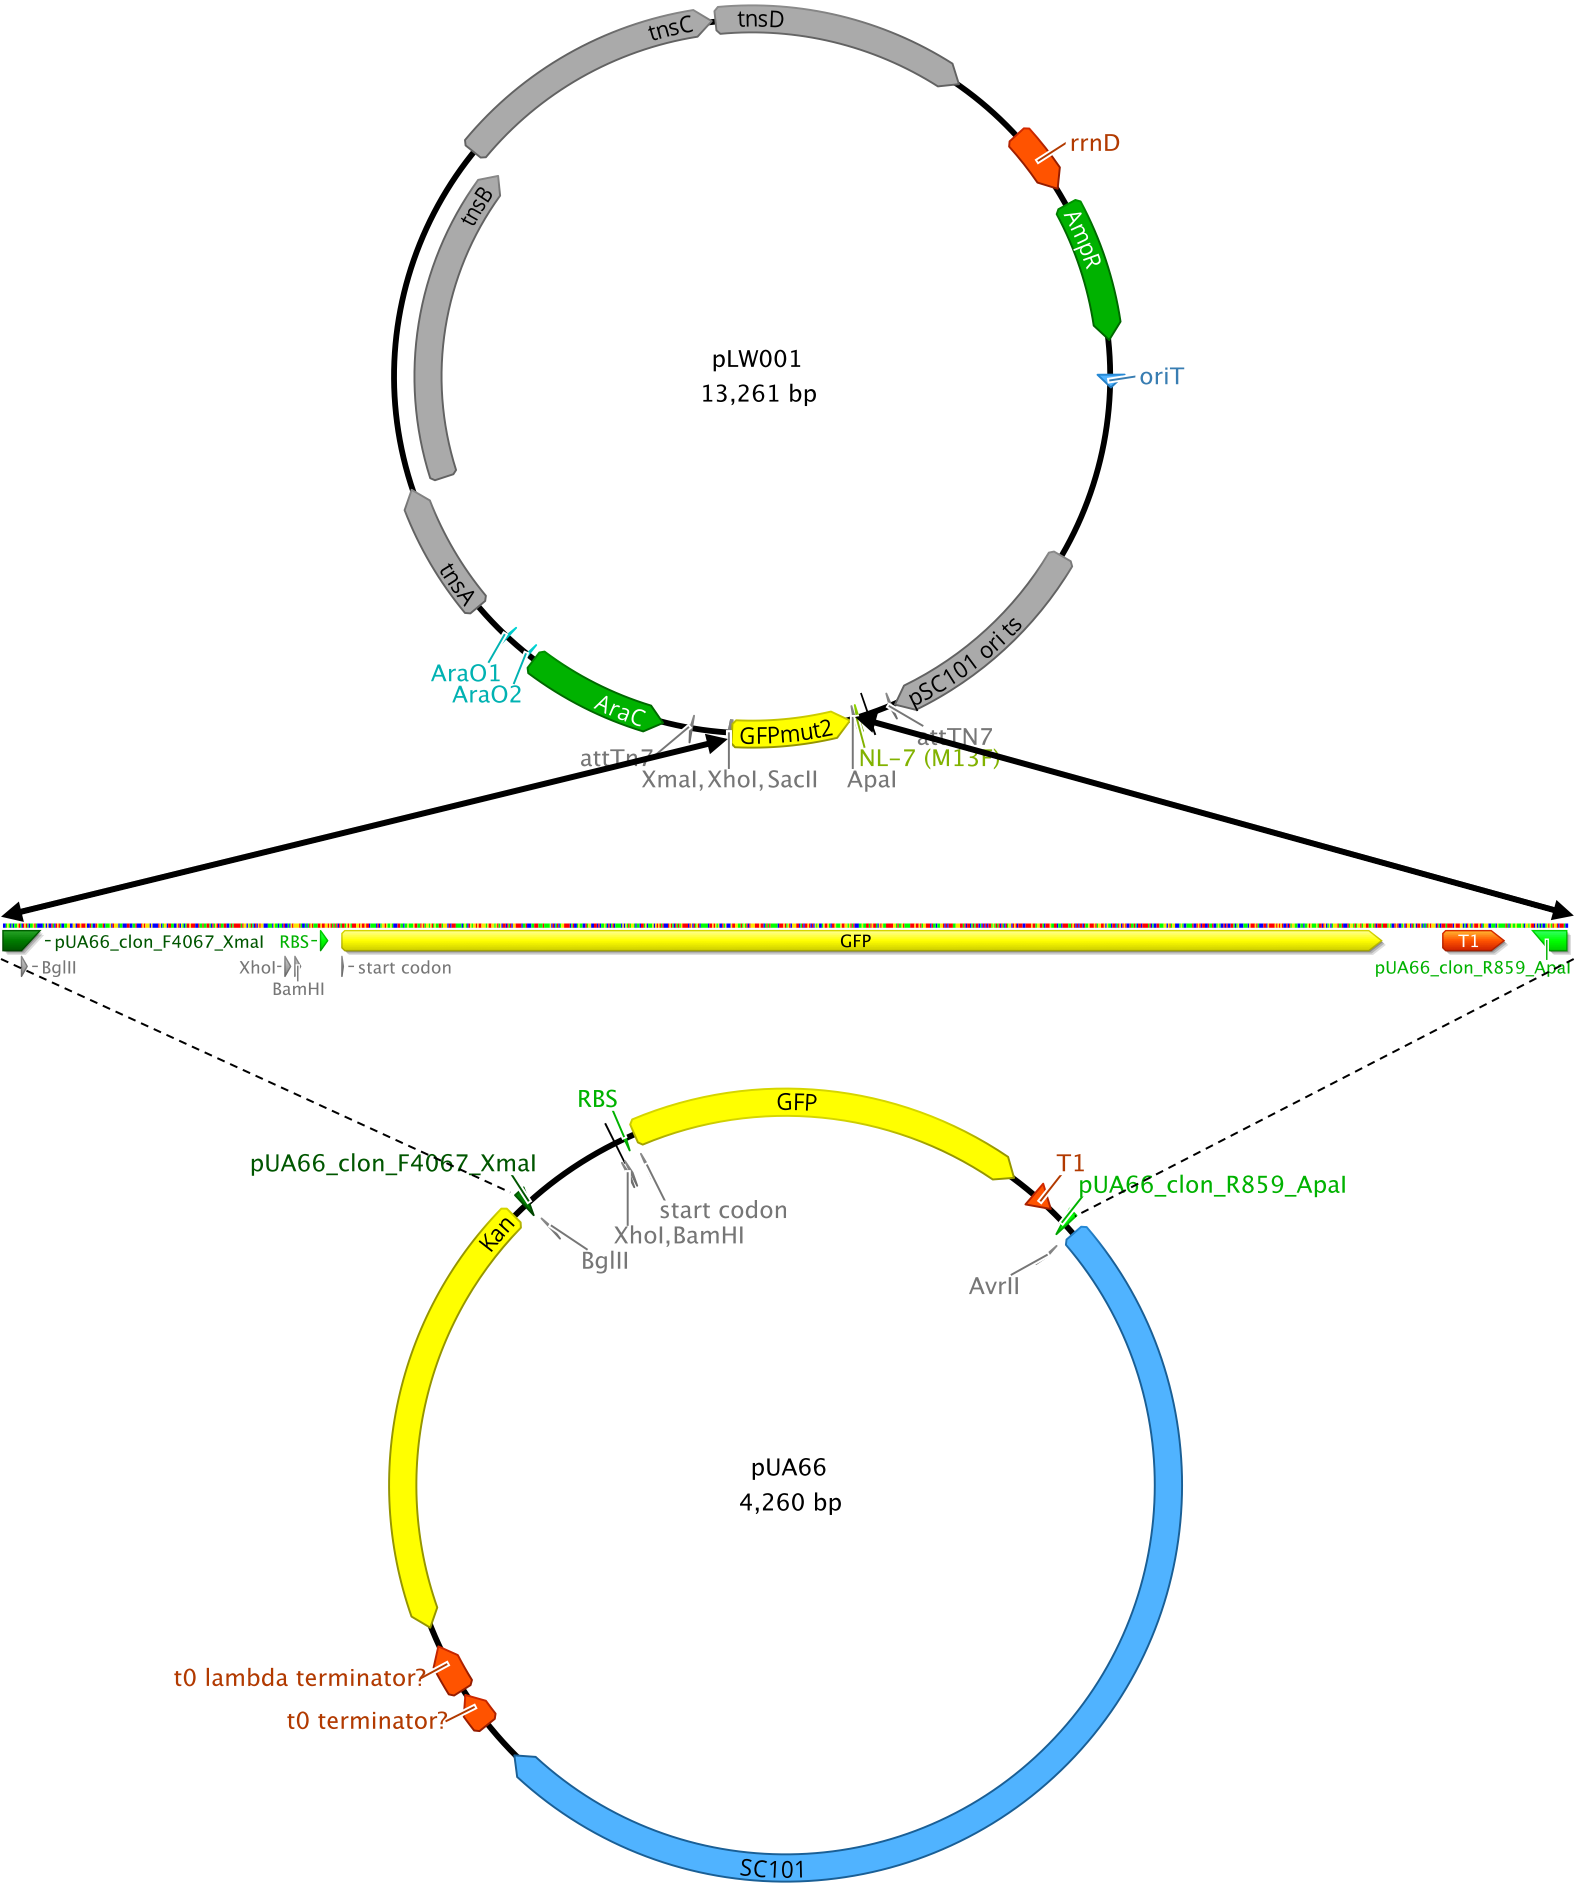
\includegraphics[scale=0.37]{text/Pictures/Cloning.png}
	\caption{Scheme of pADOUCH plasmid construction by replacing GFP sequence from pLW001 vector by sequence from pUA66 plasmid.}
	\label{cloning}
\end{figure}

We successfully amplified sequence of expected length (1.1 kb) in all 8 transformants tested (Fig. \ref{colonyPCR}), showing that successful integration had occurred.
\begin{figure}[ht!]
  \centering
  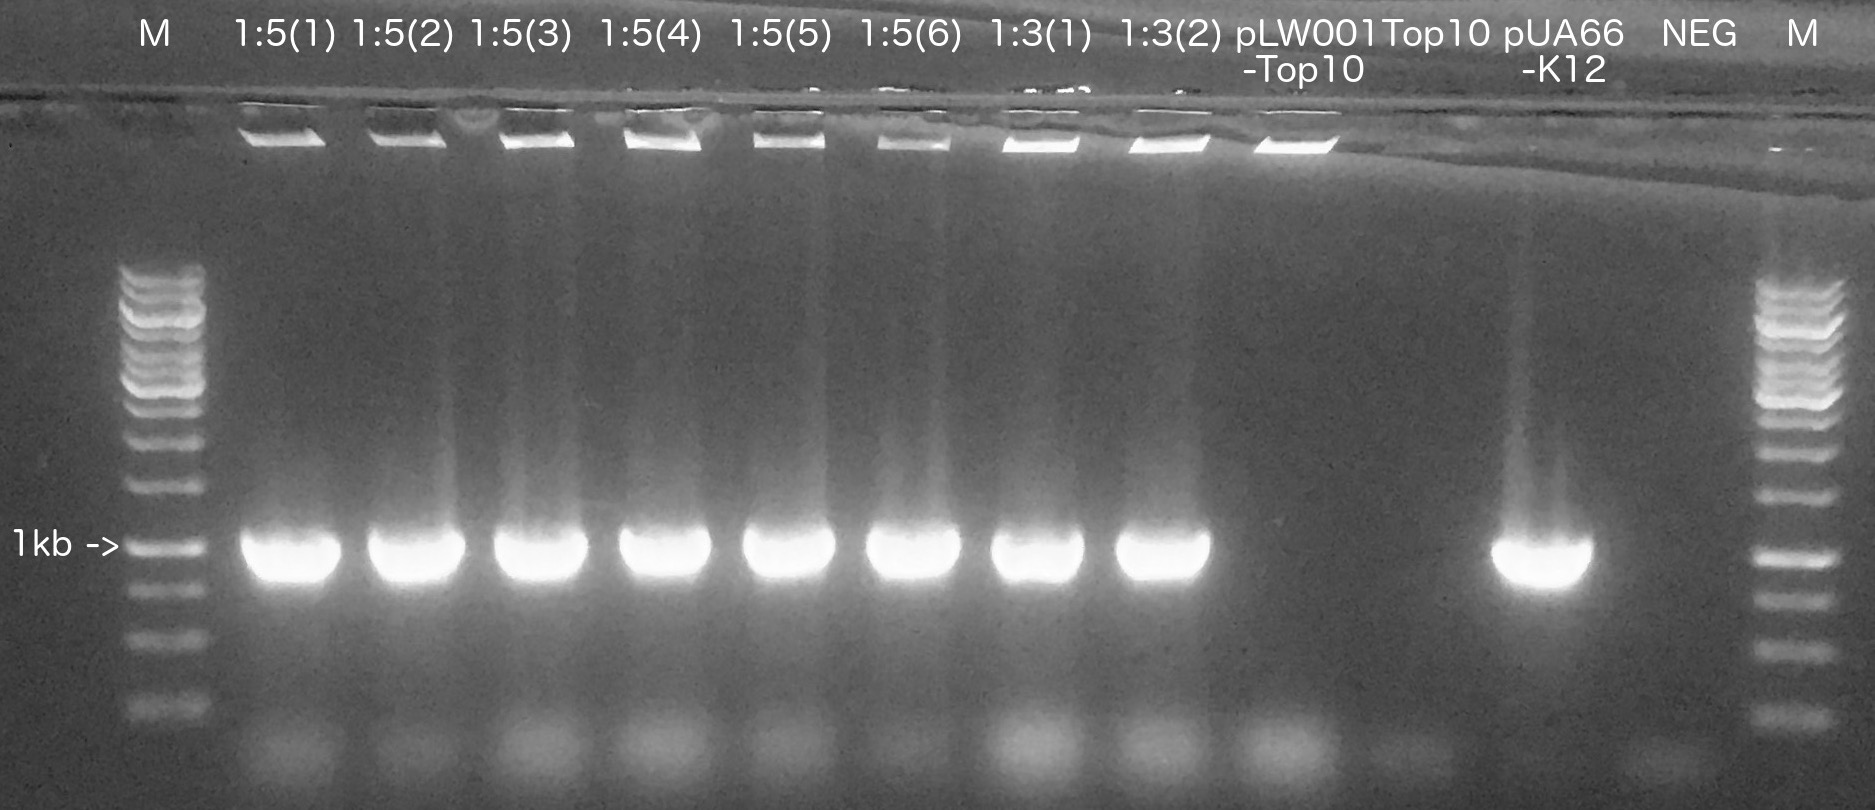
\includegraphics[scale=0.2]{text/Pictures/ColonyPCR.jpg}
	\caption{Electrophoresis of colony PCR using pUA66\textunderscore clon primers; M - marker; first 8 samples (1:5(1) - 1:3(2)) - tested clones; pLW001-Top10 and Top10 - negative controls with template DNA; pUA66-K12 - positive control; NEG - negative control without template DNA.}
	\label{colonyPCR}
\end{figure}
Sanger sequencing confirmed the presence of desired insert in digested pLW001 vector.
However, we identified four SNPs compared to the expected sequence in GFP gene (Fig. \ref{1:3(1)seq}).
But as both sequenced clones have exactly the same SNPs (\hyperlink{pADOUCHseq}{Appendix 8}) and all of these SNPs are synonymous (Fig. \ref{1:3(1)seq}), we inferred that the reference sequence of GFP gene in the pUA66 plasmid was inaccurate.
Complete revised sequence of pADOUCH vector can be found in \hyperlink{pADOUCHwhole}{Appendix 9}.
\begin{figure}[ht!]
  \centering
  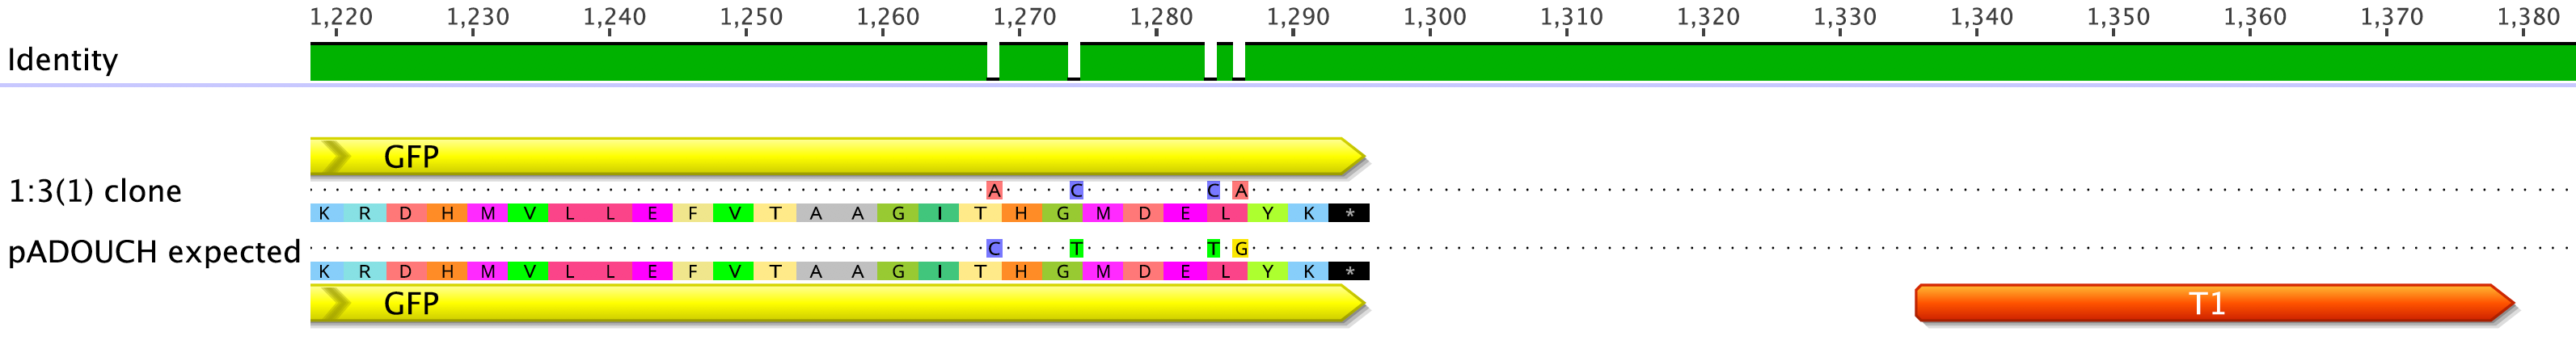
\includegraphics[scale=0.26]{text/Pictures/pADOUCHseq.png}
	\caption{Excerpt of 1:3(1) clone sequence alignment with expected pADOUCH references. DNA sequence is dotted except for SNPs; protein sequence is always beneath its DNA sequence.}
	\label{1:3(1)seq}
\end{figure}

\cleardoublepage%%% keeps correct headings

\shorthandon{-} 
%%%%%%%%%%%%%%%%%%%%%%%%%%%%%%%%%%%%


